% =====================================================================
%  rayleigh.tex -- the manual's figure of chapter 3 (Shock waves). Drawn
%  from the ME 697 Unit 5 sheet's figure (Equation_Sheets/Unit_05_rev-0/rayleigh.tex,
%  D. E. Kittell), which stays the sheet's; this copy is the manual's.
%  Built by 'make manual'.
% =====================================================================
\documentclass[tikz,border=10pt]{standalone}
\usetikzlibrary{arrows.meta}

% ---- Muted academic theme ----
\definecolor{slate}{HTML}{2C3E50}
\definecolor{oiblue}{HTML}{0072B2}
\definecolor{oiorange}{HTML}{E69F00}
\definecolor{oigreen}{HTML}{009E73}
\definecolor{oivermil}{HTML}{D55E00}

% Hugoniot: P = R0 c0^2 eta/(1-s1 eta)^2, eta = 1-V/V0, R0 c0^2 = 79.06 GPa
% Rayleigh states: strong (V/V0 = 0.713, 60 GPa), weak (0.842, 20 GPa)

\tikzset{
  axis/.style = {-{Stealth[length=6pt]}, slate, thin},
  data/.style = {oiblue, very thick},
  ray/.style  = {oivermil, line width=1.2pt},
  ray2/.style = {oivermil!50, line width=1.2pt},
}

\begin{document}
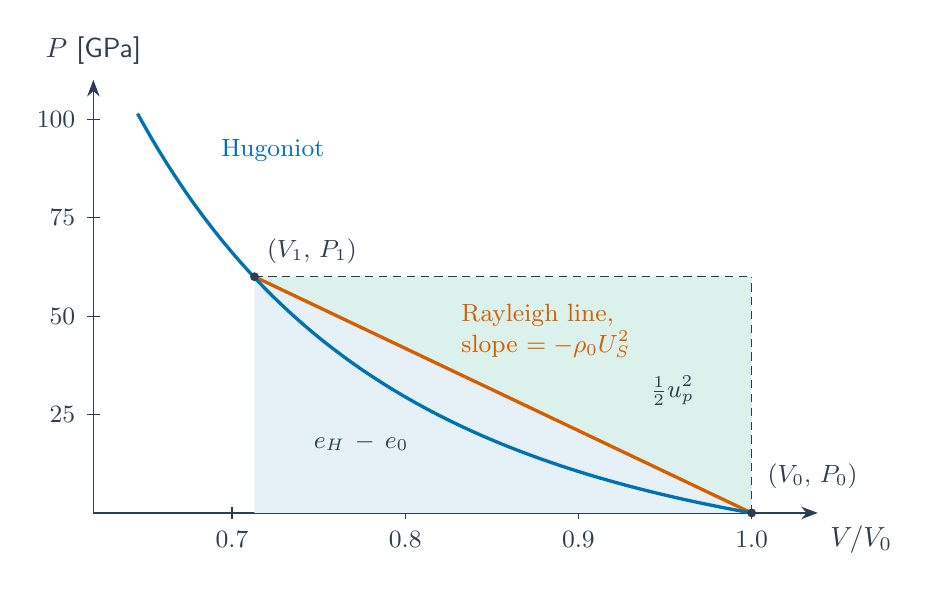
\begin{tikzpicture}[font=\sffamily, text=slate,
    declare function={
      eta(\v) = 1 - \v;
      Ph(\v)  = 79.06*eta(\v)/((1 - 1.338*eta(\v))^2);  % GPa
      X(\v)   = (\v - 0.62)*22;    % cm
      Y(\p)   = \p*0.05;           % cm
    }]

  % axes
  \draw[axis] (0,0) -- (9.2,0) node[below right=1pt] {$V/V_0$};
  \draw[axis] (0,0) -- (0,5.5) node[above=2pt] {$P$ [GPa]};

  \foreach \v/\l in {0.7/0.7, 0.8/0.8, 0.9/0.9, 1.0/1.0} {
    \draw[slate, thin] ({X(\v)}, -0.08) -- ({X(\v)}, 0.08);
    \node[below=3pt, font=\small] at ({X(\v)}, 0) {\l};
  }
  \foreach \p in {25, 50, 75, 100} {
    \draw[slate, thin] (-0.08, {Y(\p)}) -- (0.08, {Y(\p)});
    \node[left=3pt, font=\small] at (0, {Y(\p)}) {\p};
  }

  % energy partition shading (P0 = 0): below chord = internal,
  % above chord (to P = PH) = kinetic
  \fill[oiblue!10]  ({X(1.0)}, 0) -- ({X(0.713)}, 0)
                 -- ({X(0.713)}, {Y(60)}) -- cycle;
  \fill[oigreen!14] ({X(1.0)}, 0) -- ({X(0.713)}, {Y(60)})
                 -- ({X(1.0)}, {Y(60)}) -- cycle;
  \node[font=\small] at (3.4, 0.9) {$e_H\,-\,e_0$};
  \node[font=\small] at (7.35, 1.55) {$\frac{1}{2}u_p^2$};

  % Rayleigh line (chord)
  \draw[ray]  ({X(1.0)}, 0) -- ({X(0.713)}, {Y(60)});

  % Hugoniot
  \draw[data] plot[domain=0.6455:0.9995, samples=250]
      ({X(\x)}, {Y(Ph(\x))});

  % state points
  \fill[slate] ({X(1.0)}, 0) circle (1.6pt);
  \node[anchor=south west, font=\small] at ({X(1.0)+0.08}, 0.18)
      {$\left(V_0,\,P_0\right)$};
  \fill[slate] ({X(0.713)}, {Y(60)}) circle (1.6pt);
  \node[above right=1pt, font=\small] at ({X(0.713)}, {Y(60)})
      {$\left(V_1,\,P_1\right)$};

  % labels
  \node[font=\small, text=oiblue, anchor=west] at (1.5, 4.6)
      {Hugoniot};
  \node[font=\small, text=oivermil, anchor=south west, align=left]
      at (4.55, 1.85)
      {Rayleigh line,\\ slope $= -\rho_0 U_S^2$};

  % construction lines (rectangle edges, drawn last)
  \draw[slate, thin, densely dashed]
      ({X(0.713)}, {Y(60)}) -- ({X(1.0)}, {Y(60)});
  \draw[slate, thin, densely dashed]
      ({X(1.0)}, 0) -- ({X(1.0)}, {Y(60)});
\end{tikzpicture}
\end{document}
